\documentclass[12pt,spanish]{article}
\usepackage[spanish]{babel}
\usepackage{graphicx}
\usepackage{color}
\usepackage{xcolor}
\usepackage{colortbl}
\usepackage{amsthm,thmtools}
\usepackage{multirow}
\usepackage{amsmath}
\usepackage{subcaption}
\usepackage{adjustbox}
\usepackage{multirow}
\usepackage[hidelinks]{hyperref}
\usepackage{caption}
\usepackage{amsthm}
\usepackage{multicol}
\usepackage{float}
\usepackage{amsfonts}
\usepackage{titling}
\usepackage{soul}
\usepackage{listings}
\usepackage{array}
\usepackage[framemethod=tikz]{mdframed}

\graphicspath{ {../img/}}
\selectlanguage{spanish}
\usepackage[utf8]{inputenc}
\usepackage{graphicx}
\usepackage[a4paper,left=3cm,right=2cm,top=2.5cm,bottom=2.5cm]{geometry}

\newenvironment{solution}{
	\par
	\textbf{Solución}
	\par
	\begin{center}
}
{
	\end{center}
}


\title{Ingeniería de Servidores}
\setlength{\droptitle}{10em}
\author{Carlos Sánchez Páez}

\makeindex
\begin{document}
\definecolor{light-gray}{gray}{0.95}
\lstset{columns=fullflexible,basicstyle=\ttfamily}
\surroundwithmdframed[
  hidealllines=true,
  backgroundcolor=light-gray,
  innerleftmargin=0pt,
  innertopmargin=0pt,
  innerbottommargin=0pt]{lstlisting}


\begin{titlepage}

 \newlength{\centeroffset}
 \setlength{\centeroffset}{-0.5\oddsidemargin}
 \addtolength{\centeroffset}{0.5\evensidemargin}
 \thispagestyle{empty}

 \noindent\hspace*{\centeroffset}
 \begin{minipage}{\textwidth}

  \centering
  
\includegraphics[width=0.9\textwidth]{logo_ugr.jpg}\\[1.4cm]

  \textsc{ \Large Ingeniería de Servidores\\[0.2cm]}
  \textsc{GRADO EN INGENIERÍA INFORMÁTICA}\\[1cm]

  {\Huge\bfseries Resumen del temario\\}
 \end{minipage}

 \vspace{1.5cm}
 \noindent\hspace*{\centeroffset}
 \begin{minipage}{\textwidth}
  \centering

  \textbf{Autor}\\ {Carlos Sánchez Páez}\\[2.5ex]
  
\includegraphics[width=0.4\textwidth]{etsiit_logo.png}\\[0.1cm]
  \vspace{1.5cm}
  
\includegraphics[width=0.15\textwidth]{atc.jpg}\\[0.1cm]
  \vspace{1cm}
  \textsc{Escuela Técnica Superior de Ingenierías Informática y de Telecomunicación}\\
  \vspace{1cm}
  \textsc{Curso 2019-2020}
 \end{minipage}
\end{titlepage}
\thispagestyle{empty}
\newpage
\tableofcontents{}
\newpage
\listoffigures
\thispagestyle{empty}
\newpage

\section{Tema 1. Introducción a la Ingeniería de Servidores}

\subsection{¿Qué es un servidor?}

Un \textbf{sistema informático} es un conjunto de elementos \textit{hardware} (componentes físicos), \textit{software} (componentes lógicos) y \textit{peopleware} (recursos humanos) que permiote obtener, procesar y almacenar información.\\
Los sistemas informáticos se pueden clasificar atendiendo a varios factores:
\begin{itemize}
	\item Según el nivel de paralelismo (\textit{SISD},\textit{SIMD},\textit{MISD} o \textit{MIMD})
	\item Según su uso (propósito general o específico)
	\item[*] Si son servidores, según la arquitectura de servicio (sistema aislado, cliente-servidor, \emph{n} capas o cliente-cola-cliente)
\end{itemize}

\subsubsection{Según su nivel de paralelismo}

\begin{itemize}
	\item \textit{SISD}: \textbf{S}ingle \textbf{I}nstruction \textbf{S}ingle \textbf{D}ata
	\item \textit{SIMD}: \textbf{S}ingle \textbf{I}nstruction \textbf{M}ultiple \textbf{D}ata
	\item \textit{MISD}: \textbf{M}ultiple \textbf{I}nstruction  \textbf{S}ingle \textbf{D}ata
	\item \textit{MIMD}: \textbf{M}ultiple \textbf{I}nstruction  \textbf{M}ultiple \textbf{D}ata
\end{itemize}
\begin{figure}[H]
	\centering
	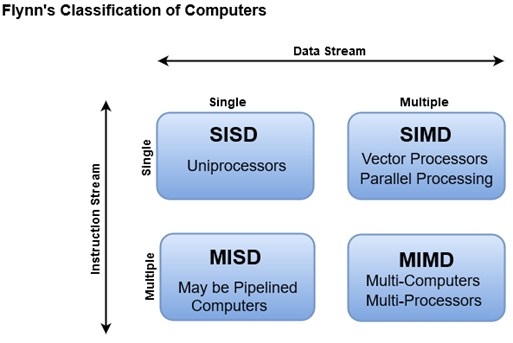
\includegraphics[width=0.5\textwidth]{comparacion_paralelismo.png}
	\caption{Sistemas informáticos según su nivel de paralelismo}
\end{figure}

\subsubsection{Según su uso}

\begin{itemize}
	\item De \textbf{uso general}: sirven para ejecutar diversas aplicaciones (PC sobremesa, portátil).
	\item De \textbf{uso específico}: ejecutan una función concreta.
	\begin{itemize}
		\item \textbf{Sistemas empotrados (\textit{embedded systems})}. Son sistemas acoplados a otro dispositivo o aparato que realizan una o varias funciones dedicadas. Suelen tener grandes restricciones de tamaño, tiempo de respuesta, etc. Ejemplo: taxímetro, cámara de vigilancia, lavadora, etc.
		\item \textbf{Servidores}. Son sistemas informáticos que forman parte de una red y proporcionan servicios a otros sistemas informáticos (clientes). Puede ser cualquier computador o \textit{clúster} (agrupación de computadores que son percibidos externamente como uno solo).
	\end{itemize}
\end{itemize}

Hay varios tipos de servidores:
\begin{itemize}
	\item \textbf{Servidor de archivos}: permite el acceso remoto a archivos almacenados o directamente accesibles por él.
	\item \textbf{Servidor web}: almacena documentos HTML, imágines, etc. y distribuye el contenido a los clientes que lo soliciten.
	\item \textbf{Servidor de base de datos}: provee servicios de base de datos a otros programas o sistemas.
	\item \textbf{Servidor de \textit{e-commerce}}: cumple o procesa transacciones comerciales. Valida al cliente y genera un pedido al servidor de bases de datos.
	\item \textbf{Servidor de impresión}: controla una o más impresoras y acepta trabajos de impresión de los clientes de la red.
	\item \textbf{Servidor de correo electrónico}: almacena, envía, recibe, etc. correos electrónicos para los clientes de la red.
\end{itemize}

\subsubsection{Según su arquitectura de servicio}
\begin{itemize}
	\item \textbf{Sistema aislado}: es un sistema que no interactúa con otros. La arquitectura es monolítica y no se distribuye la información
	\item \textbf{Arquitectura cliente-servidor}: las tareas se reparten entre los servidores (reciben solicitudes) y los clientes (remiten solicitudes). Los nodos son los servidores y los clientes.
	\item \textbf{Arquitectura cliente-servidor de \emph{n} capas}: es una arquitectura cliente-servidor que tiene \emph{n} tipos de nodos en la red, por lo que se mejora la distribución de la carga (mejorando la escalabilidad). Sus principales puntos negativos son la sobrecarga de la red que conlleva y la dificultad de programación y administración.\\
	Ejemplo de arquitectura de 3 capas:
	\begin{enumerate}
		\item Servidores que interactúan con los clientes.
		\item Servidores de \textit{e-commerce} que procesan los datos para los servidores de la capa 1.
		\item Servidores de bases de datos que buscan, gestionan y almacenan los datos para los servidores de la capa 2.
	\end{enumerate}
	\item \textbf{Arquitectura cliente-cola-cliente}: el servidor únicamente pone en contacto a los clientes y sincroniza el sistema, mientras que los clientes se encargan de cooperar para realizar la función necesaria. La arquitectura \textit{P2P} está basada en este concepto. Ejemplos: \textit{Skype}, \textit{eMule}, \textit{BitTorrent}.
\end{itemize}

\subsection{Fundamentos de la Ingeniería de Servidores}





\section{Ejercicios resueltos}
\subsection{Tema 1}
\begin{enumerate}
  \item
\end{enumerate}



\end{document}
